\subsection{进程管理}

\subsubsection{概述}
进程是操作系统中资源管理的基本单位,而线程是操作系统中调度的基本单位。在linux内核代码里,进程和线程都统一用task\_struct结构体表示。不同于linux内核,Titanix中将进程和线程分别用Process和Thread结构体表示,这样能更加清晰的处理同一进程内不同线程的创建与回收等过程。同一进程的不同线程共享地址空间(包括内核栈),后文会提到,Titanix采用无栈协程的调度方式,所有线程(包括不同进程的线程)共享同一个内核栈,调度起来开销比较小。

\subsubsection{进程控制块}

\begin{tcolorbox}[title=\textbf{os/src/process/mod.rs}]
\begin{minted}[baselinestretch=1, fontsize=\small]{rust}
/// Process control block
pub struct Process {
    /// immutable
    pid: PidHandle,
    /// mutable
    inner: SpinNoIrqLock<ProcessInner>,
}
\end{minted}
\end{tcolorbox}

我们将进程控制块分为可变和不可变的两个部分,后文会提到,进程控制块的所有权由其父进程和其包含的所有线程持有,在Rust中,对于这种有多个所有权的情况,我们需要用一个Arc(Atomic reference count)将其包裹,而Arc在Rust中默认是不可变的,因此对于可变部分,我们需要用互斥锁将其包裹;由于进程一创建便会分配一个进程ID且在其生命周期内不可变,因此我们将其归为不可变部分,对于可变部分,具体成员如下:
\begin{tcolorbox}[
title=\textbf{os/src/process/mod.rs},
listing only,
breakable
]
\begin{minted}[baselinestretch=1, fontsize=\small]{rust}
/// Process control block inner
pub struct ProcessInner {
    /// Whether this process is a zombie process
    pub is_zombie: bool,
    /// The process's address space
    pub memory_set: MemorySet,
    /// Parent process
    pub parent: Option<Weak<Process>>,
    /// Children processes
    pub children: Vec<Arc<Process>>,
    /// File descriptor table
    pub fd_table: FdTable,
    /// Allocate tid
    pub tid_allocator: RecycleAllocator,
    /// TODO: use BTreeMap to query and delete more quickly
    pub threads: Vec<Weak<Thread>>,
    /// Signal handlers for every signal
    pub sig_handler: Arc<SpinNoIrqLock<SigHandlerManager>>,
    /// Pending sigs that wait for the prcoess to handle
    pub pending_sigs: SigQueue,
    /// UStack base of all threads(the lowest bound)
    pub ustack_base: usize,
    /// Addr -> Condvar map
    pub addr_to_condvar_map: BTreeMap<usize, CondVar>,
    /// Exit code of the current process
    /// Note that we may need to put this member in every thread
    pub exit_code: i8,
    /// Current Work Directory
    /// Maybe change to Dentry later.
    pub cwd: String,
}
\end{minted}
\end{tcolorbox}
每个成员的作用如注释所述,值得注意的是,进程对所有孩子进程持有强引用(即所有权),而对父进程持有弱引用(没有所有权),这样做能防止循环引用导致内存泄漏;另外进程对其所有的线程也是持弱引用,因为某个线程可以在进程还未退出时先退出并释放内存。

\subsubsection{线程控制块}
\begin{tcolorbox}[title=\textbf{os/src/process/thread/mod.rs}]
\begin{minted}[baselinestretch=1, fontsize=\small]{rust}
/// Thread control block
pub struct Thread {
    /// immutable
    pub tid: TidHandle,
    /// the process this thread belongs to
    pub process: Arc<Process>,
    // /// whether the user specify the stack
    // pub user_specified_stack: bool,
    /// mutable
    pub inner: UnsafeCell<ThreadInner>,
}
\end{minted}
\end{tcolorbox}
类似进程控制块,我们也将线程控制块分成可变和不可变部分,不可变部分包括线程ID和该线程所属进程的Arc指针,对于可变部分,我们采用了UnsafeCell而不是像进程控制块一样采用SpinNoIrqLock,原因是UnsafeCell可以不需要加锁从而修改内部成员,顾名思义,这一行为在编译器看来是不安全的,不安全是因为编译器无法帮我们保证不同线程对该结构体的互斥访问,但对于我们的内核来说,这个成员只会在当前核心进行访问,即不可能出现在某一线程里访问另一线程的这个成员,对于这个成员,其拥有的具体子成员如下:
\begin{tcolorbox}[title=\textbf{os/src/process/thread/mod.rs}]
\begin{minted}[baselinestretch=1, fontsize=\small]{rust}
/// Thread inner,
/// This struct can only be visited by the local hart except the `terminated` field
/// which is the reason why it is an atomic variable
pub struct ThreadInner {
    // TODO: add more members
    /// Trap context that saves both kernel and user msg
    pub trap_context: TrapContext,
    /// Used for signal handle
    pub signal_context: Option<SignalContext>,
    /// When invoking `exec`, we need to get the ustack base.
    /// Note that ustack_base is the base of all ustacks
    pub ustack_base: usize,
    /// Thread state.
    /// Note that this may be modified by another thread, which
    /// need to be sync
    pub state: ThreadStateAtomic,
    /// Tid address, which may be modified by `set_tid_address` syscall
    pub tid_addr: Option<TidAddress>,
}
\end{minted}
\end{tcolorbox}
每个成员的具体作用如注释所述,值得注意的是,我们可能会出现在主线程里强制杀死别的子线程的情况,这个时候可能需要跨线程访问ThreadInner结构体并修改其state成员,因此我们将其设为原子变量,防止并发问题。

\subsubsection{线程调度}\label{schedule}

本系统的线程调度模型采用的是无栈异步协程架构, 协程即协作式多任务的子例程,协作式指的是协程的调度(挂起或运行)是由协程本身决定而不是被抢占式的;为什么说线程调度模型是协程架构呢?从用户态来说线程显然不符合协作式的概念(需要被内核抢占式调度),但从内核态来看,内核拥有线程的所有权,可以自行决定在某个时候将某个线程挂起或切换(如时钟中断的到来等),因此可以说OS中的线程对内核态来说便是协程。以下是无栈协程和有栈协程的区别:

\paragraph{有栈协程}~{}

每一个协程(即操作系统的线程)拥有自己独立的栈,每次进行协程的切换时需要修改栈指针,手动保存所有上下文信息如通用寄存器并切换为目标协程的通用寄存器,另外协程切换前后需要考虑是否有互斥锁或其他资源尚未释放,否则容易造成死锁。调度过程如\cref{pic:stack_coroutine}所示。
\begin{figure}[hbt]
    \centering
    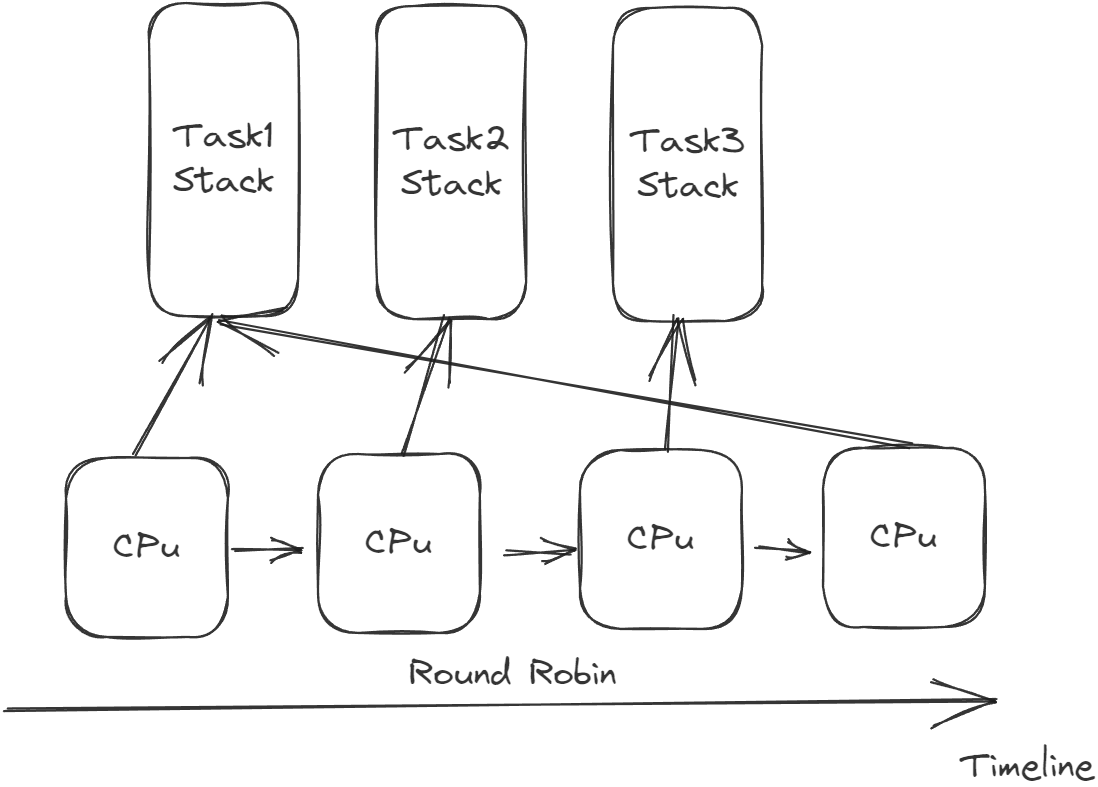
\includegraphics[width=.9\linewidth]{figure/stack_coroutine.png}
    \caption{有栈协程调度}
    \label{pic:stack_coroutine}
\end{figure}

\paragraph{无栈协程}~{}

所有的协程共用一个栈,每个协程在堆上维护一个状态机,协程的切换是通过轮询当前的状态,然后根据状态决定是否需要切换,下述代码为简单示例:

\begin{tcolorbox}[
title=\textbf{coroutine example},
listing only,
breakable
]
    \begin{minted}[baselinestretch=1, fontsize=\small]{rust}
enum PollResult {
    Ready,
    Pending,
}

enum State {
    StateA,
    StateB,
    StateC,
}

struct Coroutine {
    state: State,
}

impl Coroutine {
    pub fn poll(&mut self) -> PollResult {
        match self.state {
            State::StateA => {
                /* Do something */
                self.state = State::StateB;
                return PollResult::Pending;
            }
            State::StateB => {
                /* Do something */
                self.state = State::StateC;
                return PollResult::Pending;
            }
            State::StateC => {
                /* Do something */
                return PollResult::Ready;
            }
        }
    }
}
    \end{minted}
\end{tcolorbox}

上述代码中的poll函数即为协程的具体运行函数,不难看出其是一个状态机模型,上层每次调用poll时都可能改变其状态,从而推进其运行;总的来说,无栈协程的调度是通过函数返回然后调用另一个函数实现的,而不是像有栈协程那样直接原地更改栈指针,如下\cref{pic:nonstack_coroutine}所示。
\begin{figure}[hbt]
    \centering
    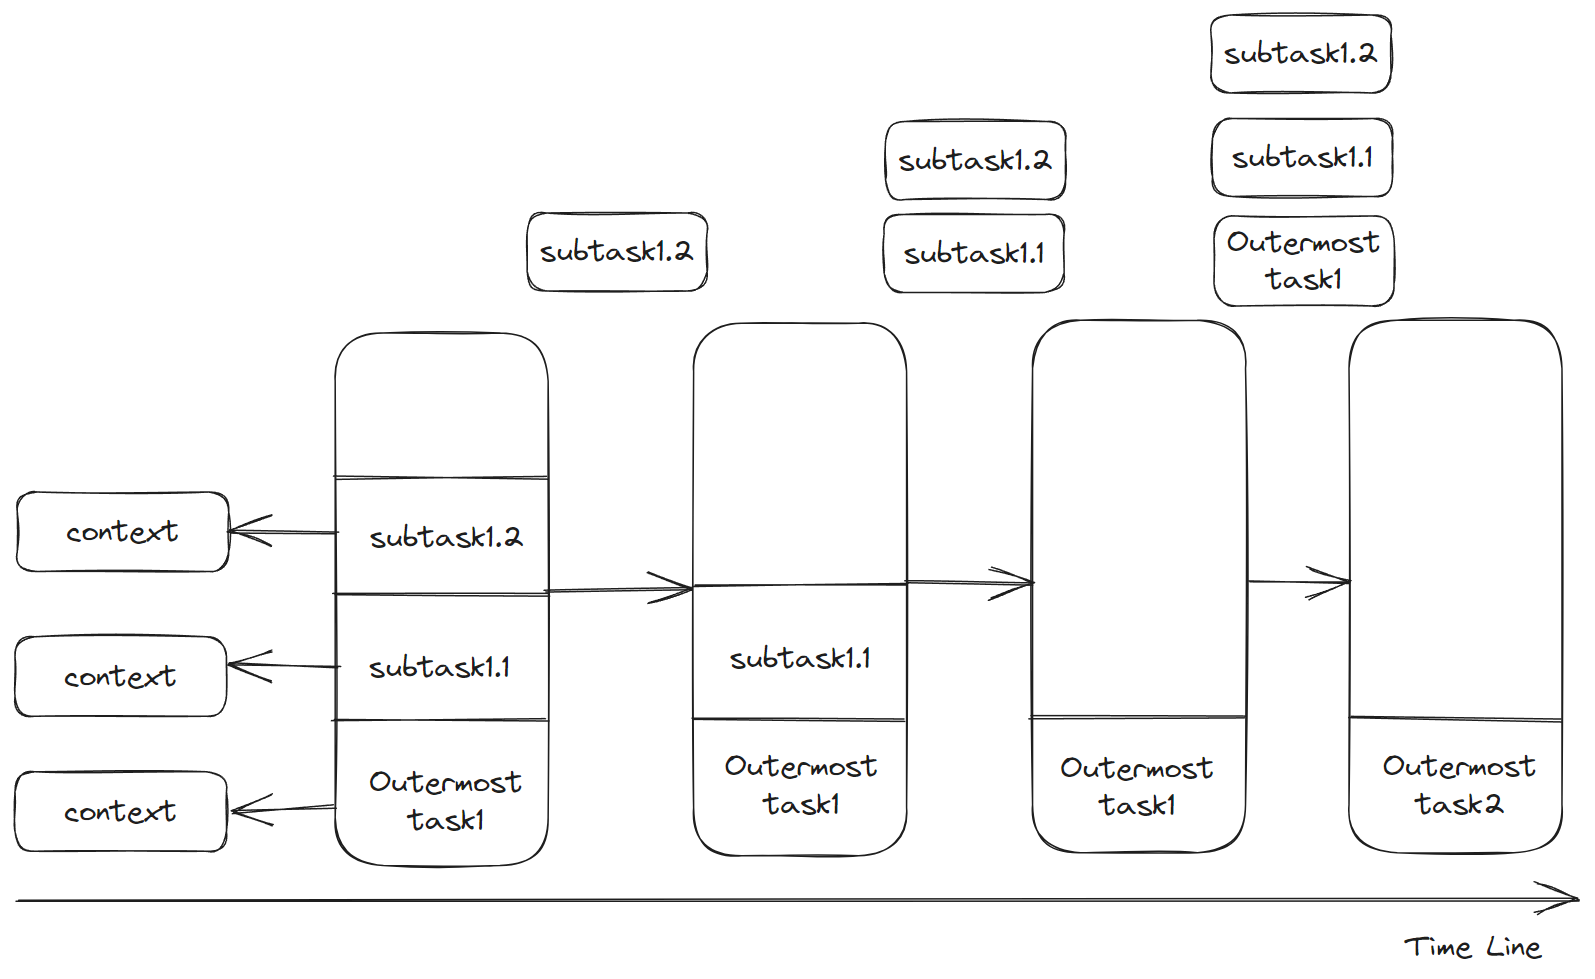
\includegraphics[width=.9\linewidth]{figure/nonstack_coroutine.png}
    \caption{无栈协程调度}
    \label{pic:nonstack_coroutine}
\end{figure}

\paragraph{Rust中的async/await}~{}

在Rust中,将一个函数定义为async或者使用async move {}包裹的代码块即为一个无栈协程,称为一个future。对于一个future,Rust会将其编译成类似上述状态机的形式,然后用户通过.await使其开始运行(即调用poll函数),因此我们可以为每一个线程设置一个future,大致框架如下:

\begin{tcolorbox}[
title=\textbf{os/src/process/thread/schedule.rs},
listing only,
breakable
]
    \begin{minted}[breaklines, baselinestretch=1, fontsize=\small]{rust}
impl<F: Future + Send + 'static> Future for UserTaskFuture<F> {
    type Output = F::Output;
    fn poll(self: Pin<&mut Self>, cx: &mut Context<'_>) -> Poll<Self::Output> {
        let this = unsafe { self.get_unchecked_mut() };
        let hart = processor::local_hart();
        
        hart.push_task(&mut this.task_ctx);
        // run the `threadloop`
        let ret = unsafe { Pin::new_unchecked(&mut this.task_future).poll(cx) };
        hart.pop_task(&mut this.task_ctx);
        
        ret
    }
}
    \end{minted}
\end{tcolorbox}

上述代码中的UserTaskFuture即为每个线程对应的无栈协程运行逻辑,在poll函数中,我们先获得当前核心(在\hyperref[multiharts]{多核心管理}中详细介绍),做一些运行新线程的准备工作(如切换页表等),然后便可以开始轮询具体的线程处理函数,每个线程的运行函数实际上是一个死循环,一直运行直至线程退出,其具体逻辑大体如下:
\begin{tcolorbox}[
title=\textbf{os/src/process/thread/threaloop.rs},
listing only,
breakable
]
    \begin{minted}[breaklines, baselinestretch=1, fontsize=\small]{rust}
pub async fn threadloop(thread: Arc<Thread>) {
    loop {
        let trap_context = unsafe {
            let p = &mut *thread.inner.get();
            &mut p.trap_context
        };
        trap::trap_return(trap_context);
        trap::trap_handler().await;
        if thread.is_zombie() {
            break;
        }
    }
    // When the process becomes zombie, all of its threads should exit too
    handle_exit(&thread);
}
    \end{minted}
\end{tcolorbox}

如上代码所示,一个线程的生命周期内做的事情就是不断重复“回到用户态执行用户态代码->由于中断或异常陷入内核进行处理”这个过程。

\paragraph{线程调度}~{}

介绍完上述关于无栈协程和Rust的async/await,我们还需要一个执行器来调度这些协程(future),这里我们采用了第三方库async-task,这个库可以构造一个future执行器来调度内核的所有任务。首先我们需要维护一个全局任务队列,然后执行器依次从全局队列中取出任务执行,只要我们的OS还有线程在跑(至少initproc永不消亡),那任务队列里就始终有任务,具体逻辑如下:
\begin{tcolorbox}[
title=\textbf{os/src/executor/mod.rs},
listing only,
breakable
]
    \begin{minted}[breaklines, baselinestretch=1, fontsize=\small]{rust}
/// Return the number of the tasks executed
pub fn run_until_idle() -> usize {
    let mut n = 0;
    loop {
        if let Some(task) = TASK_QUEUE.fetch_task() {
            // info!("fetch a task");
            task.run();
            n += 1;
        } else {
            break;
        }
    }
    n
}
    \end{minted}
\end{tcolorbox}

\paragraph{线程唤醒}~{}

Rust中的future在轮询的过程中会传入一个waker句柄,可以通过其来唤醒上层任务,我们的内核线程可以通过该句柄将某个线程唤醒,并且重新加入任务队列;

总体来看,线程调度是一个Round-Robin的过程,内核维护一个固定的时间片,每次时间片一到,会产生一个时钟中断,用户线程陷入内核,在trap\_handler函数处await出去,然后上层执行器便从任务队列中取出下一个任务,不断重复此过程即可实现分时多任务。

\subsubsection{异常与中断}
OS内核控制和调度用户程序以及各个外设硬件的方式就是异常和中断。对于RISC-V架构来说,stvec寄存器会存储中断向量,每次有异常或中断发生时,pc寄存器会被设置为stvec中存储的中断向量的值。因此我们需要做的就是实现一个异常或中断处理函数,然后将其地址存入stvec寄存器中。

\paragraph{返回用户态}~{}

返回用户态这一过程大体上来说会在两个地方用到:当一个进程在内核态被构建出来后首先要做的事情就是返回用户态去执行elf文件中的代码,此时要经历该过程;当一个进程因为异常或者中断陷入内核之后,要重新返回用户态,此时要经历该过程。由于Titanix的内核和用户共用页表,我们返回用户态的操作也比较简单。具体来说,可以把返回用户态这一步看成一个正常的函数调用,因此只需要手动保存caller-saved寄存器即可(其他寄存器会在编译的时候自动保存到内核栈中),代码如下所示:
\begin{tcolorbox}[
title=\textbf{os/src/trap/mod.rs},
listing only,
breakable
]
    \begin{minted}[breaklines, baselinestretch=1, fontsize=\small]{rust}
#[no_mangle]
/// Back to user mode.
/// Note that we don't need to flush TLB since user and
/// kernel use the same pagetable.
pub fn trap_return(trap_context: &mut TrapContext) {
    set_user_trap_entry();
    extern "C" {
        // fn __alltraps();
        fn __return_to_user(cx: *mut TrapContext);
    }

    check_signal_for_current_process();
    unsafe {
        __return_to_user(trap_context);
    }
}
    \end{minted}
\end{tcolorbox}

\_\_return\_to\_user是一个汇编函数,所做的事情就是手动保存所有的caller-saved寄存器,然后将用户态的所有通用寄存器(在下一部分 陷入内核 会讲)一并恢复,最后将TrapContext的地址保存在sscratch寄存器中。另外,值得注意的是,当一个进程刚刚被构建出来的时候,我们需要在内核态给他的用户态通用寄存器赋初值,默认是0,但栈指针需要根据我们设定的用户态栈进行赋值。

\paragraph{陷入内核}~{}

在用户因系统调用、时钟中断、缺页中断等原因发生异常和中断时,会跳转stvec中存储的中断向量,我们需要保存用户态的上下文,具体包括32个通用寄存器和sepc寄存器,当返回用户态时保存的通用寄存器可以恢复现场,sepc寄存器可以让用户态在发生异常的指令处或者下一条指令处继续执行。我们要想在中断向量中保存这些寄存器,由于此时已经处于内核态了,我们还需要一个内核结构体来保存,因此在陷入内核时需要知道该内核结构体的地址。RISC-V中有一个特权寄存器sscratch可以用来存放核心相关的上下文的地址,在前文中有提到,我们再返回用户态时会将TrapContext的地址存入sscratch中,因此这个时候便可以用其来保存用户上下文。

\paragraph{陷阱处理函数}~{}

由于我们的内核是异步的,结合了Rust的async/await机制,因此自然要将陷进处理函数(即trap handler)定义为异步函数,实际上,内核的进程切换点也是在trap handler中。

具体来说,我们在trap handler中对不同的中断或异常类型进行相应的处理,对于每种情况,可能的结果有:
\begin{enumerate}
    \item 正常处理并返回用户态;
    \item 发生用户态严重异常,导致进程直接退出,不会再返回用户态;
    \item 时钟中断,当前进程切换到下一个进程(严格来说是线程),此时该进程会一直等到下一次调度到自己后才返回用户态;
\end{enumerate}

\subsubsection{多核心管理}\label{multiharts}
对于RISC-V架构来说,每个核心有自己独立的一套寄存器,因此从总体上看,只需要给每个核心划分好内核栈,便可以开始进行并行调度运行,多核内存管理在下一章节讨论。这里我们重点关注多核运行,前面\hyperref[schedule]{线程调度}中提到,每次取出新的任务时,我们需要拿到当前的核心,而我们将每个核心的核心控制块地址存放在tp寄存器中,因此可以通过读取tp寄存器来获取当前核心,核心控制块的定义如下:
\begin{tcolorbox}[
title=\textbf{os/src/processor/hart.rs},
listing only,
breakable
]
    \begin{minted}[breaklines, baselinestretch=1, fontsize=\small]{rust}
pub struct Hart {
    hart_id: usize,
    /// Spare env ctx when in need(e.g. kernel thread or idle thread)
    spare_env_ctx: EnvContext,
    local_ctx: LocalContext,
    /// Every hart has its own kernel stack
    kstack_bottom: usize,
}
    \end{minted}
\end{tcolorbox}
核心控制块的关键成员在于local\_ctx成员,该成员可以在挂上各种各样的per-CPU的成员,目前有栈追踪器(用来记录调用栈)、页表和线程控制块,线程控制块即当前核心正在运行的线程,每次调度新的任务时需要修改satp值以启用新的页表,同时刷新TLB。